% 第 XVIII 讲第 3 节；原 PDF 374—391 页，第 374 页自第 3 节标题起。
\SourcePage{374}
\SGAsection{3}{整体对偶定理}
\textbf{3.1. \Term{functor}{函子} $Rf^!$。}我们需要\Term{canonical}{典范}\Term{flasque-resolution}{松弛解消}的一种变式。

\begin{SGAresult}{引理}{3.1.1}
设 $X$ 是一个\Term{coherent-scheme}{凝聚概形}（即\Term{quasi-compact}{拟紧}且\Term{quasi-separated}{拟分离}）。\Term{functor}{函子} $\varinjlim$ 给出如下两\Term{category}{范畴}之间的\Term{equivalence}{等价}：\Term{constructible-sheaf}{可构造}\Term{set}{集合}\Term{sheaf}{层}（分别为群\Term{sheaf}{层}、\Term{abelian-group}{阿贝尔群}\Term{sheaf}{层}）\Term{category}{范畴}的\Term{ind-object}{Ind 对象}\Term{category}{范畴}，以及\Term{set}{集合}\Term{sheaf}{层}（分别为 Ind \Term{finite-group}{有限群}\Term{sheaf}{层}、\Term{torsion-sheaf}{挠阿贝尔层}）的\Term{category}{范畴}。
\end{SGAresult}
这由第 IX 讲 2.7.2 和第 IX 讲 2.7.3 得到。

\textbf{3.1.2.} 设 $F$ 是\Term{scheme}{概形} $X$ 上的\Term{torsion-sheaf}{挠阿贝尔层}，它是\Term{constructible-sheaf}{可构造层} $(F_i)_{i\in I}$ 的\Term{filtered-colimit}{滤过归纳极限}；设 $X_0$ 是 $X$ 的一个\Term{conservative-points}{保守点集}。用公式
\[
 C^*_{\ell}(F)=\varinjlim_i C^*(F_i)
\]
定义 $F$ 的\Term{modified-canonical-flasque-resolution}{修正典范松弛解消}；这里 $C^*(F_i)$ 是第 XVII 讲 4.2.2 中的\Term{canonical}{典范}\Term{flasque-resolution}{松弛解消}。由 3.1.1，当 $X$ \Term{coherent-scheme}{凝聚}时，此定义不依赖 $F_i$ 的选择。它还与\Term{localization}{局部化}交换；借助这一事实，对于任意\Term{scheme}{概形} $X$（不必\Term{coherent-scheme}{凝聚}）上的\Term{torsion-sheaf}{挠层} $F$，可由整体化定义 $C^*_{\ell}(F)$。

\Term{complex}{复形} $C^*_{\ell}(F)$ 是 $F$ 的一个\Term{resolution}{解消}，对 $F$ 具有\Term{functorial}{函子性}；其构造与\Term{localization}{局部化}及\Term{filtered-colimit}{滤过归纳极限}交换；\Term{functor}{函子} $C^n_{\ell}$ 是\Term{exact-functor}{正合的}。

由此，对于 $X$ 上的\Term{sheaf-of-rings}{环层} $A$，\Term{functor}{函子} $C^n_{\ell}$ 将 $A$-\Term{module}{模}变为 $A$-\Term{module}{模}；它们同样将\Term{torsion-sheaf}{挠层}变为\Term{torsion-sheaf}{挠层}。下面的事实众所周知。

\begin{SGAresult}{引理}{3.1.3}
设 $\mathscr A$ 是一个有小生成集的 $\mathcal U$-\Term{abelian-category}{阿贝尔范畴}，且以小\Term{filtered-ordered-set}{滤过有序集}为指标的\Term{colimit}{归纳极限}在 $\mathscr A$ 中\Term{representable}{可表}且\Term{exact}{正合}。\Term{functor}{函子} $\mathsf F\colon\mathscr A^\circ\to(\mathrm{Ens})$
\SourcePage{375}
\Term{representable}{可表}的充分必要条件是：它将任意小\Term{colimit}{归纳极限}变为\Term{projective-limit}{投射极限}。
\end{SGAresult}
例如参见 SGA 4 第 I 讲 8.12.5；那里既不假设 $\mathscr A$ 是\Term{abelian-category}{阿贝尔范畴}，也不假设\Term{filtered}{滤过} $\varinjlim$ \Term{exact}{正合}。

我们将把此引理用于\Term{ringed-site}{赋环景} $(X,A)$ 上\Term{module-sheaf}{模层}的\Term{category}{范畴} $\operatorname{Mod}(X,A)$。在此特例中，若\Term{functor}{函子} $\mathsf F$ 由\Term{sheaf}{层} $\underline F$ \Term{representable}{表示}，则
\[
 \underline F(U)=\mathsf F(A_U).\tag{3.1.3.1}
\]
借助 $\underline F$ 的这一描述，可在所考虑的情形直接证明 3.1.3。

回顾：若 $f\colon X\to S$ 是\Term{compactifiable-morphism}{可紧化态射}（第 XVII 讲 3.2），则 $S$ \Term{quasi-compact}{拟紧}且\Term{quasi-separated}{拟分离}（原文如此），并且 $f$ 的\Term{fibre}{纤维}\Term{dimension}{维数}\Term{bounded}{有界}。

\begin{SGAresult}{定理}{3.1.4}
设 $f\colon X\to S$ 是\Term{compactifiable-morphism}{可紧化态射}，$A$ 是 $S$ 上的\Term{torsion-ring-sheaf}{挠环层}。则\Term{functor}{函子}
\[
 Rf_!\colon D(X,f^*A)\longrightarrow D(S,A)\tag{3.1.4.1}
\]
有一个部分定义的\Term{right-adjoint}{右伴随函子}
\[
 Rf^!\colon D^+(S,A)\longrightarrow D^+(X,f^*A):\tag{3.1.4.2}
\]
对于 $K\in\operatorname{Ob}D(X,f^*A)$ 和 $L\in\operatorname{Ob}D^+(S,A)$，有\Term{functorial}{函子性}\Term{isomorphism}{同构}
\[
 \operatorname{Hom}(Rf_!K,L)\simeq\operatorname{Hom}(K,Rf^!L).\tag{3.1.4.3}
\]
赋予此\Term{functor}{函子}使下图\Term{commutative-diagram}{交换}的\Term{translation-morphism}{平移态射}：
\begin{equation}\tag{3.1.4.4}
\begin{tikzcd}[column sep=small]
\operatorname{Hom}(Rf_!(K[1]),L) \arrow[r,leftrightarrow,"\sim"] \arrow[d,leftrightarrow,"\wr"'] &
\operatorname{Hom}(K[1],Rf^!L)\simeq\operatorname{Hom}(K,(Rf^!L)[-1]) \arrow[d,leftrightarrow,"\wr"]\\
\operatorname{Hom}((Rf_!K)[1],L)\simeq\operatorname{Hom}(Rf_!K,L[-1]) \arrow[r,leftrightarrow,"\sim"',"\text{伴随}" ] &
\operatorname{Hom}(K,Rf^!(L[-1]))
\end{tikzcd}
\end{equation}
则 $Rf^!$ 是一个\Term{triangulated-functor}{三角函子}。
\end{SGAresult}
\textbf{注意。}记号 $Rf^!$ 有些滥用，因为一般说来，$Rf^!$ 并不是某个\Term{functor}{函子} $f^!$ 的\Term{derived-functor}{导出函子}。

\begin{proof}
取整数 $d$，使 $f$ 的每个\Term{fibre}{纤维}的\Term{dimension}{维数}都 $<d$，并选择一个\Term{compactification}{紧化}
\[
\begin{tikzcd}
 X\arrow[r,hook,"j"]\arrow[d,"f"'] &\overline X\arrow[dl,"\overline f"]\\ S &
\end{tikzcd}
\]
\SourcePage{376}
若 $K$ 是 $X$ 上的 $f^*A$-\Term{module}{模}\Term{complex}{复形}，则
\[
 Rf_!K\simeq R\overline f_*(j_!K).
\]
对 $X$ 上任意\Term{sheaf}{层} $F$，\Term{complex}{复形} $\tau_{\leq2d}C^*_{\ell}j_!F$ 的各\Term{set-component}{分量} $F^i$ 满足
\[
 R^k\overline f_*F^i=0\qquad(k>0).\tag{3.1.4.5}
\]
事实上，当 $i\ne2d$ 时，$F^i$ 是\Term{flasque-sheaf}{松弛层}的\Term{colimit}{归纳极限}；当 $i=2d$ 且 $k>0$ 时，由第 XVII 讲 5.2.8.1，
\[
 R^k\overline f_*F^{2d}=R^{k+2d}f_!F=0.
\]
与 $K$ 的\Term{truncation}{截断}\Term{modified-canonical-flasque-resolution}{修正典范松弛解消}这一\Term{double-complex}{双复形}相伴的\Term{simple-complex}{单复形}是 $K$ 的\Term{resolution}{解消}。所以由 (3.1.4.5)，按第 XVII 讲 1.1.15 的记号，有
\[
 R\overline f_*(j_!K)\xleftarrow{\sim}\overline f_*\tau_{\leq2d}''C^*_{\ell}j_!K.\tag{3.1.4.6}
\]
记 $f_!^\bullet$ 为从 $X$ 上\Term{module-sheaf}{模层}到 $S$ 上\Term{sheaf}{层}\Term{complex}{复形}的\Term{functor}{函子}，定义为
\[
 f_!^\bullet(F)=\overline f_*\tau_{\leq2d}C^*_{\ell}j_!F.\tag{3.1.4.7}
\]
\begin{SGAresult}{引理}{3.1.4.8}
(i) \Term{functor}{函子} $f_!^i$ \Term{exact-functor}{正合}且与\Term{filtered-colimit}{滤过归纳极限}交换；当 $i\notin[0,2d]$ 时 $f_!^i=0$。

(ii) \Term{functor}{函子} $f_!^\bullet$ \Term{bounded}{有界}且各\Term{set-component}{分量}\Term{exact}{正合}，因而可平凡地\Term{derive}{导出}（第 XVII 讲 1.2.10）为
\[
 Rf_!^\bullet\quad\text{或简记为}\quad f_!^\bullet\colon D(X,f^*A)\to D(S,A).
\]
\Term{arrow}{箭头} (3.1.4.6) 是\Term{functor}{函子}\Term{isomorphism}{同构}
\[
 Rf_!^\bullet\xrightarrow{\sim}Rf_!.
\]
\end{SGAresult}
\Term{functor}{函子} $C^i_{\ell}$ \Term{exact-functor}{正合}且与\Term{filtered-colimit}{滤过归纳极限}交换（3.1.2）。它们将任意\Term{sheaf}{层}变成\Term{acyclic-sheaf}{无环层}。\Term{functor}{函子} $\overline f_*$ 与 $j_!$ 与\Term{filtered-colimit}{滤过归纳极限}交换。由此得到：

a) \Term{functor}{函子} $\overline f_*C^i_{\ell}j_!$，从而\Term{functor}{函子} $f_!^i$，都与\Term{filtered-colimit}{滤过归纳极限}交换；

b) 当 $i<2d$ 时，\Term{functor}{函子} $f_!^i=\overline f_*C^i_{\ell}j_!$ \Term{exact-functor}{正合}。当 $i=2d$ 时，由 (3.1.4.5) 可知 $f_!^i$ \Term{exact-functor}{正合}。

3.1.4.8 中其余断言是显然的。

\textbf{注记 3.1.4.9。} $f_!^\bullet$ 的定义不依赖\Term{sheaf-of-rings}{环层} $A$，并且对任意阿贝尔\Term{sheaf}{层}仍有意义。断言 3.1.4.8 (i) 在 $X$ 与 $S$ 上\Term{torsion-sheaf}{挠阿贝尔层}的\Term{category}{范畴}中仍然成立。

\SourcePage{377}
由 3.1.4.8 和 3.1.3，\Term{functor}{函子}
\[
 f_!^i\colon\operatorname{Mod}(X,f^*A)\longrightarrow\operatorname{Mod}(S,A)
\]
有\Term{right-adjoint}{右伴随函子} $f_i^!$；由于 $f_!^i$ \Term{exact-functor}{正合}，$f_i^!$ 将\Term{injective-object}{内射对象}变为\Term{injective-object}{内射对象}。

采用第 XVII 讲 1.1.12 的\Term{signature}{符号}约定，\Term{functor}{函子} $f_i^!$ 构成一个\Term{left-exact-functor}{左正合函子}\Term{complex}{复形}，在\Term{cohomological-degree}{上同调次数} $n\notin[-2d,0]$ 时为零：
\[
 f^{!\bullet}\colon\operatorname{Mod}(S,A)\longrightarrow C^b(X,f^*A).\tag{3.1.4.10}
\]
\Term{functor}{函子} $f^{!\bullet}$ 可\Term{derive}{导出}（第 XVII 讲 1.2.10）为\Term{triangulated-functor}{三角函子}
\[
 Rf^!\colon D^+(S,A)\longrightarrow D^+(X,f^*A),\tag{3.1.4.11}
\]
它\Term{right-adjoint}{右伴随}于\Term{functor}{函子} $Rf_!$（$=Rf_!^\bullet=Lf_!^\bullet$）（“平凡的\Term{duality}{对偶}公式”）。更确切地说，若 $I\in\operatorname{Ob}C^+(S,A)$ 是一个由\Term{injective-object}{内射} $A$-\Term{module-sheaf}{模层}组成的\Term{complex}{复形}，则 $A$-\Term{module}{模} $f_i^!I^n$ 是\Term{injective-object}{内射的}，且有三重\Term{complex}{复形}\Term{isomorphism}{同构}（第 XVII 讲 1.1.12）
\[
 \operatorname{Hom}^\bullet(f_!^\bullet K,I)\xrightarrow{\sim}
 \operatorname{Hom}^\bullet(K,f^{!\bullet}I).\tag{3.1.4.12}
\]
取相伴\Term{simple-complex}{单复形}（用乘积计算）的 $H^0$，便得到\Term{adjunction}{伴随}断言。相容性 (3.1.4.4) 留给读者验证。
\end{proof}

\textbf{注记 3.1.5。} 假定\Term{functor}{函子} $Rf^!$ 具有\Term{finite}{有限}\Term{cohomological-amplitude}{上同调振幅}。由第 XVII 讲 1.2.10，\Term{functor}{函子} $f^{!\bullet}$ 此时有\Term{derived-functor}{导出函子}
\[
 Rf^!\colon D(S,A)\longrightarrow D(X,A).\tag{3.1.5.1}
\]
此\Term{derived-functor}{导出函子}仍\Term{right-adjoint}{右伴随}于\Term{functor}{函子} $Rf_!$ (3.1.4.1)。事实上，有
\begin{align*}
\operatorname{Hom}_{D(S)}(Rf_!K,L)
 &\simeq\varinjlim_{L\xrightarrow{\sim}L'}\operatorname{Hom}_{K(S)}(f_!^\bullet K,L')\\
 &\simeq\varinjlim_{\substack{K'\xrightarrow{\sim}K\\L\xrightarrow{\sim}L'}}\operatorname{Hom}_{K(S)}(f_!^\bullet K',L'),\\
\operatorname{Hom}_{D(X)}(K,Rf^!L)
 &\simeq\varinjlim_{K'\xrightarrow{\sim}K}\operatorname{Hom}_{K(X)}(K',Rf^!L)\\
 &\simeq\varinjlim_{\substack{K'\xrightarrow{\sim}K\\L\xrightarrow{\sim}L'}}\operatorname{Hom}_{K(X)}(K',f^{!\bullet}L'),
\end{align*}
又由\Term{adjunction}{伴随}，
\begin{align*}
\operatorname{Hom}_{K(S)}(f_!^\bullet K',L')
 &=H^0\operatorname{Hom}(f_!^\bullet K',L')\\
 &\simeq H^0\operatorname{Hom}(K',f^{!\bullet}L')
 =\operatorname{Hom}_{K(X)}(K',L').
\end{align*}

\begin{SGAresult}{定义}{3.1.6}
\Term{triangulated-functor}{三角函子}
\[
 Rf^!\colon D^+(S,A)\longrightarrow D^+(X,f^*A)
\]
（或在 3.1.5 的假设下，
\[
 Rf^!\colon D(S,A)\longrightarrow D(X,f^*A)\text{）},
\]
它\Term{right-adjoint}{右伴随}于\Term{functor}{函子} $Rf_!$ (3.1.4.1)，称为\Term{extraordinary-inverse-image}{例外逆像函子}。
\end{SGAresult}

\SourcePage{378}
\begin{SGAresult}{命题}{3.1.7}
设\Term{compactifiable-morphism}{可紧化态射} $f\colon X\to S$ 的\Term{relative-dimension}{相对维数} $\leq d$。

(i) 若 $L\in\operatorname{Ob}D^+(S,A)$ 满足 $H^i(L)=0$（$i\leq k$），则 $H^iRf^!L=0$（$i\leq k-2d$）。

(ii) 对 $L\in\operatorname{Ob}D^b(S,A)$，有
\[
 \operatorname{dim\,inj}(Rf^!L)\leq\operatorname{dim\,inj}(L).
\]
\end{SGAresult}
\Term{functor}{函子} $Rf^!$ 是 $f^{!\bullet}\colon\operatorname{Mod}(S,A)\to C^b\operatorname{Mod}(X,f^*A)$ 的\Term{right-derived-functor}{右导出函子}。断言 (i) 来自 $(f^{!\bullet})^i=0$（$i<-2d$）；断言 (ii) 来自 $(f^{!\bullet})^i=0$（$i>0$）以及\Term{functor}{函子} $f_i^!$ 将\Term{injective-object}{内射对象}变为\Term{injective-object}{内射对象}。

\begin{SGAresult}{命题}{3.1.8}
设 $f\colon X\to S$ 是\Term{quasi-finite}{拟有限}的\Term{compactifiable-morphism}{可紧化态射}。

(i) \Term{functor}{函子} $f_!\colon\operatorname{Mod}(X,f^*A)\to\operatorname{Mod}(S,A)$ 有\Term{right-adjoint}{右伴随函子} $f^!\colon\operatorname{Mod}(S,A)\to\operatorname{Mod}(X,f^*A)$，而 $Rf^!$ 是\Term{functor}{函子} $f^!$ 的\Term{derived-functor}{导出函子}。

(ii) 若 $f$ 是\Term{closed-immersion}{闭浸入}，则 $f^!$ 是“\Term{support}{支集}在 $X$ 中的\Term{section}{截面}”\Term{functor}{函子}。

(iii) 若 $f$ \Term{etale}{平展}，则 $f^!$ 与\Term{functor}{函子} $f^*$ 等同，且以
\[
 \operatorname{Tr}_f\colon f_!f^*F\longrightarrow F
\]
为\Term{adjunction-morphism}{伴随态射}。
\end{SGAresult}
断言 (i) 立即来自 3.1.4 证明中 $d=0$ 的特例：此时 $f_!^\bullet=f_!$ 且 $f^{!\bullet}=f^!$。\Term{equivalence}{等价}地，\Term{adjoint-functor}{伴随函子} $f^!$ 的存在由 3.1.3 及 $f_!$ \Term{exact-functor}{正合}且与\Term{filtered-colimit}{滤过归纳极限}交换得到；\Term{adjunction}{伴随} $(f_!,Rf^!)$ 是一个“平凡的\Term{duality}{对偶}公式”。断言 (ii) 是显然的，而 (iii) 就是第 XVII 讲 6.2。

\textbf{3.1.9.} 设 $f\colon X\to S$ 是\Term{compactifiable-morphism}{可紧化态射}，$A$ 是 $S$ 上的\Term{torsion-ring-sheaf}{挠环层}，并以 $A$ 的\Term{inverse-image}{逆像}给 $X$ \Term{ringed}{赋环}。设 $K\in\operatorname{Ob}D^-(X,f^*A)$，$L\in\operatorname{Ob}D^+(X,f^*A)$；以一个\Term{bounded-below}{下有界}的\Term{injective-sheaf}{内射层}\Term{complex}{复形}表示 $L$，于是
\[
 R\mathscr Hom(K,L)\simeq\mathscr Hom(K,L).
\]
\Term{complex}{复形} $\mathscr Hom(K,L)$ 的各\Term{set-component}{分量}均为\Term{flasque-sheaf}{松弛层}，所以
\[
 Rf_*R\mathscr Hom(K,L)\simeq f_*\mathscr Hom(K,L).\tag{3.1.9.1}
\]
\SourcePage{379}
如 3.1.4 的证明，选择 $f$ 的一个\Term{compactification}{紧化}和整数 $d$，由此得到\Term{functor}{函子} $f_!^\bullet$ (3.1.4.7)。
\begin{equation}\tag{3.1.9.2}
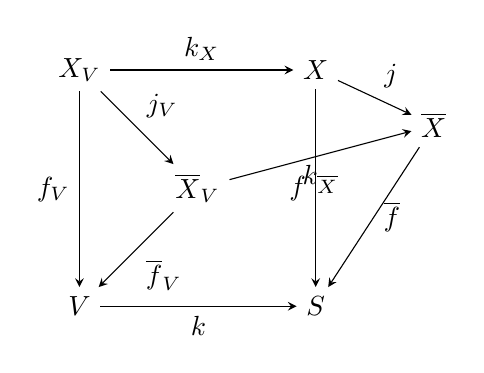
\begin{tikzpicture}[>=stealth,baseline=(current bounding box.center)]
\node (xv) at (0,3) {$X_V$};\node (x) at (3,3) {$X$};
\node (bv) at (1.5,1.5) {$\overline X_V$};\node (b) at (4.5,2.3) {$\overline X$};
\node (v) at (0,0) {$V$};\node (s) at (3,0) {$S$};
\draw[->] (xv)--node[above]{$k_X$}(x);\draw[->] (xv)--node[left]{$f_V$}(v);
\draw[->] (x)--node[left]{$f$}(s);\draw[->] (v)--node[below]{$k$}(s);
\draw[->] (xv)--node[above right]{$j_V$}(bv);\draw[->] (x)--node[above right]{$j$}(b);
\draw[->] (bv)--node[below]{$k_{\overline X}$}(b);\draw[->] (bv)--node[below right]{$\overline f_V$}(v);
\draw[->] (b)--node[right]{$\overline f$}(s);
\end{tikzpicture}
\end{equation}
对每个 $V\in\operatorname{Ob}S_{\text{ét}}$，有\Term{isomorphism}{同构}
\[
 k^*f_!^\bullet\xrightarrow{\sim}f_{V!}^\bullet k_X^*,\tag{3.1.9.3}
\]
从而
\[
 \mathscr Hom^\bullet(f_!^\bullet K,f_!^\bullet L)(V)
 \simeq\mathscr Hom^\bullet\bigl(f_{V!}^\bullet(k_X^*K),f_{V!}^\bullet(k_X^*L)\bigr).
\]
$f_{V!}^\bullet$ 的\Term{functorial}{函子性}给出
\[
\begin{split}
 \mathscr Hom^\bullet(K,L)(X_V)&=\operatorname{Hom}^\bullet(k_X^*K,k_X^*L)\\
 &\longrightarrow\operatorname{Hom}^\bullet\bigl(f_{V!}^\bullet(k_X^*K),f_{V!}^\bullet(k_X^*L)\bigr),
\end{split}
\]
因而在\Term{complex}{复形}层次给出\Term{arrow}{箭头}
\[
 f_*\mathscr Hom^\bullet(K,L)\longrightarrow
 \mathscr Hom^\bullet(f_!^\bullet K,f_!^\bullet L).\tag{3.1.9.4}
\]
由 (3.1.9.1)，此\Term{arrow}{箭头}可\Term{derive}{导出}为
\[
 Rf_*R\mathscr Hom(K,L)\longrightarrow
 R\mathscr Hom(Rf_!K,Rf_!L).\tag{3.1.9.5}
\]
现在设 $K\in\operatorname{Ob}D^-(X,A)$，$L\in\operatorname{Ob}D^+(S,A)$。由从 $Rf_!Rf^!L$ 到 $L$ 的\Term{adjunction-morphism}{伴随箭头}及 (3.1.9.4)，得到复合\Term{arrow}{箭头}
\[
\begin{split}
 Rf_*R\mathscr Hom(K,Rf^!L)&\longrightarrow
 R\mathscr Hom(Rf_!K,Rf_!Rf^!L)\\
 &\longrightarrow R\mathscr Hom(Rf_!K,L),
\end{split}
\]
这是\Term{adjunction-isomorphism}{伴随同构}在 $S$ 上的\Term{local-scheme}{局部}\Term{form}{形式}：
\[
 Rf_*R\mathscr Hom(K,Rf^!L)\longrightarrow
 R\mathscr Hom(Rf_!K,L).\tag{3.1.9.6}
\]
\begin{SGAresult}{命题}{3.1.10}
\Term{arrow}{箭头} (3.1.9.6) 是\Term{isomorphism}{同构}。
\end{SGAresult}
\SourcePage{380}
设 $V\in\operatorname{Ob}S_{\text{ét}}$，沿用 (3.1.9.2) 的记号。\Term{isomorphism}{同构}（“\Term{transitivity}{传递性}”）
\[
 k_!Rf_{V!}\simeq Rf_!k_{X!},
\]
其存在是\Term{functor}{函子} $Rf^!$ 理论的\Term{jacobson-radical}{根基}，经\Term{transpose}{转置}得到\Term{localization-isomorphism}{局部化同构}（3.1.8 (iii)）
\[
 k_X^*Rf^!\simeq Rf_V^!k^*,\tag{3.1.10.1}
\]
它在\Term{complex}{复形}层次由一个\Term{morphism}{态射}表示：
\[
 k_X^*f^{!\bullet}\longrightarrow f_V^{!\bullet}k^*.
\]
要证明 (3.1.9.6) 是\Term{isomorphism}{同构}，只需证明对每个 $V\in\operatorname{Ob}S_{\text{ét}}$，(3.1.9.6) 都诱导\Term{isomorphism}{同构}
\[
\begin{split}
 \operatorname{Hom}(k_X^*K,k_X^*Rf^!L)
 &\simeq H^0(V,Rf_*R\mathscr Hom(K,Rf^!L))\\
 &\longrightarrow H^0(V,R\operatorname{Hom}(Rf_!K,L))\\
 &\simeq\mathscr Hom(k^*Rf_!K,k^*L).
\end{split}\tag{3.1.10.2}
\]
当 $V=X$ 时，这正是 (3.1.4.3)。一般情形由下列相容性得到；\emph{编写者并未核实此相容性}：
\begin{SGAresult}{引理}{3.1.10.3}
下图\Term{commutative-diagram}{交换}：
\[
\begin{tikzcd}[column sep=large]
\operatorname{Hom}(k_X^*K,k_X^*Rf^!L)\arrow[r,"{(3.1.10.2)}"]\arrow[d,"\wr"',"{(3.1.10.1)}"] &\operatorname{Hom}(k^*Rf_!K,k^*L)\arrow[d,"\wr","\text{局部化}"']\\
\operatorname{Hom}(k_X^*K,Rf_V^!k_X^*L)\arrow[r,leftrightarrow,"\sim"',"{(3.1.4.3)\text{ 在 }V\text{ 上}}"] &\operatorname{Hom}(Rf_!k^*K,k^*L)
\end{tikzcd}
\]
\end{SGAresult}

\textbf{3.1.11.} 设有\Term{cartesian-square}{笛卡尔方块}
\begin{equation}\tag{3.1.11.1}
\begin{tikzcd}
X'\arrow[r,"g'"]\arrow[d,"f'"']&X\arrow[d,"f"]\\
S'\arrow[r,"g"']&S,
\end{tikzcd}
\end{equation}
其中 $f$ \Term{compactifiable-morphism}{可紧化}，$A$ 是 $S$ 上的\Term{torsion-ring-sheaf}{挠环层}，$B$ 是 $S'$ 上的\Term{torsion-ring-sheaf}{挠环层}，$M$ 是\Term{bounded-above}{上有界}的 $(f^*A,B)$-\Term{bimodule}{双模}\Term{complex}{复形}。此时，在\Term{complex}{复形}层次有关于 $K$（$K\in\operatorname{Ob}C(X,f^*A)$）的\Term{functor}{函子}\Term{morphism}{态射}
\[
 M\otimes_Ag^*f_!^\bullet K\longrightarrow
 f_!^{\prime\bullet}(f'^*M\otimes_Ag'^*K),\tag{3.1.11.2}
\]
\SourcePage{381}
它经\Term{transpose}{转置}成为关于 $L$（$L\in\operatorname{Ob}C(S',B)$）的\Term{functor}{函子}\Term{morphism}{态射}
\[
 g'_*\mathscr Hom_B(f'^*M,f^{\prime!\bullet}L)
 \longrightarrow f^{!\bullet}g_*\operatorname{Hom}_B(M,L).\tag{3.1.11.3}
\]
此\Term{morphism}{态射}可\Term{derive}{导出}为从 $D^+(S',B)$ 到 $D^+(X,f^*A)$ 的、关于 $L$ 的\Term{functor}{函子}\Term{morphism}{态射}：
\[
 Rg'_*R\mathscr Hom_B(f'^*M,Rf'^!L)
 \longrightarrow Rf^!Rg_*R\operatorname{Hom}_B(M,L),\tag{3.1.11.4}
\]
它使下图\Term{commutative-diagram}{交换}；其中 $K\in\operatorname{Ob}D^-(X,f^*A)$，$L\in\operatorname{Ob}D^+(S',B)$：
\[
\resizebox{\linewidth}{!}{$
\begin{tikzcd}[ampersand replacement=\&,column sep=small,row sep=large]
\operatorname{Hom}(K,Rg'_*R\mathscr Hom_B(f'^*M,Rf'^!L))
 \arrow[r,"\text{\textcircled{1}}"]\arrow[d,leftrightarrow]
 \&\operatorname{Hom}(K,Rf^!Rg_*R\operatorname{Hom}_B(M,L))
 \arrow[r,leftrightarrow,"\text{伴随}"]
 \&\operatorname{Hom}(Rf_!K,Rg_*R\operatorname{Hom}_B(M,L))\arrow[d,leftrightarrow]\\
\operatorname{Hom}(g'^*K,R\mathscr Hom_B(f'^*M,Rf'^!L))\arrow[d,leftrightarrow]
 \&\&\operatorname{Hom}(g^*Rf_!K,R\operatorname{Hom}_B(M,L))\arrow[d,leftrightarrow]\\
\operatorname{Hom}(f'^*M\otimes_Ag'^*K,Rf'^!L)
 \arrow[r,leftrightarrow,"\text{伴随}"]
 \&\operatorname{Hom}(Rf'_!(f'^*M\otimes_A^Lg'^*K),L)
 \arrow[r,"\text{\textcircled{2}}"]
 \&\operatorname{Hom}_B(M\otimes_A^Lg^*Rf_!K,L).
\end{tikzcd}$}
\]
此图中，\textcircled{2}（由第 XVII 讲 5.2.2.1 的\Term{arrow}{箭头}得到）是\Term{isomorphism}{同构}（第 XVII 讲 5.2.6）。所以对任意 $K$，\Term{arrow}{箭头}\textcircled{1}都是\Term{isomorphism}{同构}，这就推出 (3.1.11.4) 是\Term{isomorphism}{同构}。

因此，\Term{proper}{固有态射}的\Term{base-change-theorem}{基变换定理}经\Term{transpose}{转置}得到：
\begin{SGAresult}{命题}{3.1.12}
\Term{arrow}{箭头} (3.1.11.4) 是\Term{isomorphism}{同构}。
\end{SGAresult}
称此\Term{isomorphism}{同构}为\Term{induction-isomorphism}{诱导同构}。下面列出它的三个特例。

\begin{SGAresult}{推论}{3.1.12.1}
设 $f\colon X\to S$ 是\Term{compactifiable-morphism}{可紧化态射}，$A$、$B$ 是 $S$ 上的两个\Term{torsion-ring-sheaf}{挠环层}，$\varphi\colon B\to A$ 是\Term{homomorphism}{同态}。用 $\rho$ 表示从 $B$ 到 $A$ 的\Term{restriction-of-scalars}{标量限制}。则对 $K\in\operatorname{Ob}D^+(S,B)$，有
\[
 \rho Rf^!K\xrightarrow{\sim}Rf^!(\rho K).
\]
\end{SGAresult}
只需在 (3.1.11.3) 中取 $S=S'$，$X=X'$，$A=A$，$B=B$，$M=A$。

由此可见，\Term{sheaf-of-rings}{环层}在 $Rf^!$ 的构造中所起的\Term{action}{作用}只是一个幌子。

\begin{SGAresult}{推论}{3.1.12.2}
设 $f\colon X\to S$ 是\Term{compactifiable-morphism}{可紧化态射}，$A$ 是 $S$ 上的\Term{torsion-ring-sheaf}{挠环层}，$K\in\operatorname{Ob}D^-(S,A)$，$L\in\operatorname{Ob}D^+(S,A)$。有\Term{induction-formula}{诱导公式}
\[
 R\mathscr Hom(f^*K,Rf^!L)\xrightarrow{\sim}Rf^!R\mathscr Hom(K,L)
\]
（取 $S=S'$，$X=X'$）。
\end{SGAresult}

\SourcePage{382}
\begin{SGAresult}{推论}{3.1.12.3}
对于每个 3.1.11 中的方块和每个 $L\in\operatorname{Ob}D^+(S',A)$，有
\[
 Rg'_*Rf'^!L\xrightarrow{\sim}Rf^!Rg_*L
\]
（取 $B=f^*A=M$）。
\end{SGAresult}

\textbf{3.1.13.} 对 $S$-\Term{compactifiable-morphism}{可紧化态射}的复合 $gh$
\[
 X\xrightarrow{h}Y\xrightarrow{g}Z,
\]
\Term{composition-isomorphism}{复合同构}
\[
 c_{g,h}\colon Rg_!Rh_!\xrightarrow{\sim}R(gh)_!
\]
经\Term{transpose}{转置}成为\Term{composition-morphism}{复合态射}
\[
 c^!_{g,h}\colon Rh^!Rg^!\xrightarrow{\sim}R(gh)^!,\tag{3.1.13.1}
\]
它对三重复合满足通常的\Term{cocycle-condition}{上闭链条件}。换言之，各\Term{category}{范畴} $D^+(X,f^*A)$ 构成一个\Term{fibred-and-cofibered-category}{纤维且余纤维范畴}的各\Term{fibre}{纤维}，其底\Term{category}{范畴}的\Term{object}{对象}是 $S$-\Term{scheme}{概形} $f\colon X\to S$，\Term{arrow}{箭头}是 $S$-\Term{compactifiable-morphism}{可紧化态射}；\Term{direct-image}{直接像}（分别为\Term{inverse-image}{逆像}）\Term{functor}{函子}就是 $Rf_!$（分别为 $Rf^!$）。因此，对每个\Term{compactifiable-morphism}{可紧化态射}的\Term{commutative-square}{交换方块}
\[
\begin{tikzcd}
X'\arrow[r,"g"]\arrow[d,"f'"']&X\arrow[d,"f"]\\
S'\arrow[r,"g'"']&S,
\end{tikzcd}
\]
都有\Term{cobase-change-morphism}{余基变换态射}（第 XVII 讲 2.1.3）
\[
 \operatorname{ch}^!\colon Rf'_!Rg^!\longrightarrow Rg'^!Rf_!.\tag{3.1.13.2}
\]

\textbf{3.1.14.} 设有\Term{cartesian-square}{笛卡尔方块}
\[
\begin{tikzcd}
X'\arrow[r,"g'"]\arrow[d,"f'"']&X\arrow[d,"f"]\\
S'\arrow[r,"g"']&S,
\end{tikzcd}
\]
其中 $f$ \Term{compactifiable-morphism}{可紧化}；设 $A$ 是 $S$ 上的\Term{torsion-ring-sheaf}{挠环层}。以 $A$ 的\Term{inverse-image}{逆像}给 $S'$、$X$ 和 $X'$ \Term{ringed}{赋环}，仍滥用记号将这些\Term{inverse-image}{逆像}记为 $A$。\Term{base-change-isomorphism}{基变换同构}
\[
 g^*Rf_!\xrightarrow{\sim}Rf'_!g'^*\tag{3.1.14.1}
\]
\SourcePage{383}
使我们能把\Term{category}{范畴} $D(S,A)$、$D(X,A)$、$D(S',A)$ 和 $D(X',A)$ 看成如下\Term{commutative-diagram}{交换图}的\Term{category}{范畴}上的一个\Term{cofibered-category}{余纤维范畴}的各\Term{fibre}{纤维}：
\[
\begin{tikzcd}
X\arrow[d]&X\arrow[l]\arrow[d]\\
X&X\arrow[l]
\end{tikzcd}
\]
其\Term{direct-image}{直接像}\Term{functor}{函子}为 $Rf_!$、$Rf'_!$、$g^*$ 和 $g'^*$（原文如此）。\Term{restriction}{限制}到各 $D^+$ \Term{category}{范畴}，甚至得到此图上的一个\Term{fibred-and-cofibered-category}{纤维且余纤维范畴}，其\Term{direct-image}{直接像}\Term{functor}{函子}为 $Rf^!$、$Rf'^!$、$Rg_*$ 和 $Rg'_*$（原文如此）。由此得到：

a) 对于“\Term{inverse-image}{逆像}”\Term{functor}{函子}，有“\Term{transitivity-isomorphism}{传递同构}”（原文如此）
\[
 Rg_*Rf^!\xrightarrow{\sim}Rf^!Rg_*,
\]
这在 3.1.12.3 中已经得到（同样以 (3.1.14.1) 的\Term{transpose}{转置}来定义）。

b) 有一个“\Term{base-change-morphism}{基变换态射}”（第 XVII 讲 2.1.3）
\[
 g'^*Rf^!\longrightarrow Rf'^!g^*,\tag{3.1.14.2}
\]
根据所引之处，可用下列两种方式描述它：

a) 由\Term{adjunction}{伴随}，给定一个\Term{morphism}{态射} (3.1.14.2) \Term{equivalence}{等价}于给定\Term{morphism}{态射}
\[
 Rf'_!g'^*Rf^!\longrightarrow g^*.
\]
\Term{base-change-theorem}{基变换定理}通过以下复合给出这样一个\Term{morphism}{态射}：
\[
 Rf'_!g'^*Rf^!\xleftarrow{\sim}g^*Rf_!Rf^!
 \xrightarrow{g^*\ast\mathrm{adj.}}g^*.
\]

b) 由\Term{adjunction}{伴随}，给定一个\Term{morphism}{态射} (3.1.14.2) \Term{equivalence}{等价}于给定\Term{morphism}{态射}
\[
 Rf^!\longrightarrow Rg'_*Rf'^!g^*.
\]
\Term{isomorphism}{同构} (3.1.12.3) 通过以下复合给出这样一个\Term{morphism}{态射}：
\[
 Rf^!\xrightarrow{Rf^!\ast\mathrm{adj.}}Rf^!Rg_*g^*
 \xleftarrow{\sim}Rg'_*Rf'^!g^*.
\]
根据这些\Term{morphism}{态射}在\Term{fibred-and-cofibered-category}{纤维且余纤维范畴}中的解释，显然 (3.1.12.3)、(3.1.13.2) 和 (3.1.14.2) 中的\Term{morphism}{态射}，各自对于 $f$ 或 $g$ 是两个\Term{morphism}{态射}的复合的情形，均满足两个第 XII 讲 4.4 型的相容性。

下面的一般\Term{topology}{拓扑}结果将在下一小节中使用。

\SourcePage{384}
\textbf{3.1.15.} 设 $f\colon X\to S$ 是\Term{site-morphism}{景态射}。用 $\Gamma(f)$ 表示如下的\Term{site}{景}。

a) \Term{category}{范畴} $\Gamma(f)$ 是由三元组 $(U,V,\varphi)$ 构成的\Term{category}{范畴}，其中
\[
 U\in\operatorname{Ob}(X),\quad V\in\operatorname{Ob}S,\quad
 \varphi\in\operatorname{Hom}(X,\varphi^*V).
\]

b) 一族\Term{morphism}{态射} $(u_i,v_i)\colon(U_i,V_i,\varphi_i)\to(U,V,\varphi)$ 是\Term{covering-family}{覆盖族}，当且仅当在 $X$ 中各\Term{morphism}{态射} $u_i\colon U_i\to U$ \Term{cover}{覆盖} $U$。

于是有：

\textbf{3.1.15.1.} 从 $\Gamma(f)$ 到 $X$ 的\Term{functor}{函子}
\[
 (U,V,\varphi)\longmapsto U
\]
是一个\Term{site-equivalence}{景等价} $\gamma\colon X\to\Gamma(f)$。

\textbf{3.1.15.2.} 从 $S$ 到 $\Gamma(f)$ 的\Term{functor}{函子} $f_\Gamma^*$
\[
 V\longmapsto(f^*V,V,\operatorname{Id}_{f^*V})
\]
是一个\Term{site-morphism}{景态射}，记为 $f_\Gamma\colon\Gamma(f)\to S$，或滥用记号简记为 $f$。它满足 $f_\Gamma\gamma\simeq f$。\Term{functor}{函子} $f_\Gamma^*$ 有\Term{right-adjoint}{右伴随函子} $f_{\Gamma\bullet}$：
\[
 f_{\Gamma\bullet}\colon(U,V,\varphi)\longmapsto V.
\]
因此\Term{functor}{函子} $f_{\Gamma\bullet}$ 是从 $\Gamma(f)$ 到 $S$ 的\Term{site-comorphism}{景余态射}，并且与\Term{site-morphism}{景态射} $f_\Gamma^*$ 定义相同的\Term{topos-morphism}{拓扑斯态射}。
\begin{equation}\tag{3.1.15.3}
\begin{tikzcd}[column sep=large]
X&\Gamma(f)\arrow[l,"*"',"\approx"]\arrow[dl,bend left=12,"f_{\Gamma\bullet}"]\\
S\arrow[u,"f^*"]\arrow[ur,bend left=12,"f_\Gamma^*"]&
\end{tikzcd}
\end{equation}
由此得到以下计算\Term{sheaf}{层}的\Term{inverse-image}{逆像}的规则。

\textbf{3.1.15.4.} 设 $F$ 是 $S$ 上的\Term{sheaf}{层}，$f_\Gamma^\bullet F$ 是 $\Gamma(f)$ 上由下式给出的\Term{presheaf}{预层}：
\[
 f_\Gamma^\bullet F(U,V,\varphi)=F(V),
\]
而 $af_\Gamma^\bullet F$ 是它生成的\Term{sheaf}{层}。则
\[
 f^*F(U)\simeq af_\Gamma^\bullet F(U,V,\varphi).
\]

\textbf{3.1.16.} 设 $f\colon X\to S$ 是\Term{site-morphism}{景态射}，$A$ 是 $S$ 上的\Term{sheaf-of-rings}{环层}，$B$ 是 $X$ 上的\Term{sheaf-of-rings}{环层}，$d$ 是一个整数。设 $K$ 是下述类型的\Term{object}{对象}。

\SourcePage{385}
\textbf{3.1.16.1.} $K$ 为 $X$ 的每个\Term{object}{对象} $U$ 指定一个 $S$ 上的 $(A,f_*(B|U))$-\Term{module}{模}\Term{complex}{复形} $K(U)$，它在次数 $>d$ 时为零；且 $K(U)$ 是 $U$ 的\Term{covariant-functor}{协变函子}。

对每个 $S$ 上的 $A$-\Term{module-sheaf}{模层} $F$，以 $K^!F$ 表示由如下 $B$-\Term{module}{模}\Term{presheaf}{预层}\Term{complex}{复形}生成的 $X$ 上\Term{sheaf}{层}\Term{complex}{复形}：
\[
 U\longmapsto\operatorname{Hom}_A(K(U),F).
\]
用 $RK^!$ 表示 $K^!$ 的\Term{derived-functor}{导出函子}：
\[
 RK^!\colon D^+(S,A)\longrightarrow D^+(X,B).
\]
若 $U\colon K_1\to K_2$ 是 (3.1.11.1) 型\Term{object}{对象}的\Term{morphism}{态射}，则 $U$ 诱导\Term{functor}{函子}\Term{morphism}{态射}
\[
 {}^tu\colon K_2^!\longrightarrow K'_1,\qquad
 RK_2^!\longrightarrow RK_1^!.
\]
在上述假设下，有：

\begin{SGAresult}{命题}{3.1.17}
(i) 对每个 $X$ 的点 $x$ 及每个 $L\in\operatorname{Ob}D^+(S,A)$，以 $\mathcal V(x)$ 表示 $x$ 的\Term{neighbourhood}{邻域}\Term{category}{范畴}，则有
\[
 H^n(RK^!L)_x\simeq\varinjlim_{U\in\operatorname{Ob}\mathcal V(x)}
 \operatorname{Ext}^n(K(U),L).\tag{3.1.17.1}
\]

(ii) 因此，有\Term{spectral-sequence}{谱序列}
\[
 E_2^{pq}=\varinjlim_{U\in\operatorname{Ob}\mathcal V(x)}
 \operatorname{Ext}^p(H^{-q}(K(W)),L)\Longrightarrow H^n(K^!L)_x.\tag{3.1.17.2}
\]

(iii) 若 $X^0$ 是 $X$ 的一个\Term{conservative-points}{保守点集}，$u\colon K_1\to K_2$ 是 (3.1.11.1) 型\Term{object}{对象}的\Term{morphism}{态射}，则
\[
 {}^tu\colon RK_2^!\longrightarrow RK_1^!
\]
为\Term{isomorphism}{同构}的充分必要条件是：对每个 $n$ 和每个 $x\in X^0$，$\operatorname{Mod}(S,A)$ 中的\Term{pro-object}{pro 对象}\Term{morphism}{态射}
\[
 u_x\colon\text{``}\varprojlim_{U\in\operatorname{Ob}\mathcal V(x)}\text{''}\,H^nK_1(U)
 \longrightarrow\text{``}\varprojlim_{U\in\operatorname{Ob}\mathcal V(x)}\text{''}\,H^nK_2(U)\tag{3.1.17.3}
\]
是\Term{isomorphism}{同构}。
\end{SGAresult}
\begin{proof}
为证明 (i)，取 $L$ 为一个\Term{injective-object}{内射对象}\Term{complex}{复形}，则 (3.1.17.1) 是显然的；显然 (i) $\Rightarrow$ (ii)。

(iii) 中条件 (3.1.17.3) 的充分性立即由 (3.1.17.2) 得到。我们无需使用其必要性。若 ${}^tu$ 是\Term{isomorphism}{同构}，则由 (3.1.16.1)，对 $(S,A)$ 上每个\Term{injective-sheaf}{内射层} $I$，有
\[
\operatorname{Hom}\bigl(\text{``}\varprojlim_{\mathcal V(x)}\text{''}\,H^nK_2(U),I\bigr)
 \xrightarrow{\sim}
\operatorname{Hom}\bigl(\text{``}\varprojlim_{\mathcal V(x)}\text{''}\,H^nK_1(U),I\bigr),
\]
\SourcePage{386}
注意在任何有足够多\Term{injective-object}{内射对象}的\Term{abelian-category}{阿贝尔范畴} $\mathscr A$ 中（这里是 $\operatorname{Mod}(S,A)$），各\Term{functor}{函子} $\operatorname{Hom}(x,I)$（$I$ 遍历 $\mathscr A$ 的\Term{injective-object}{内射对象}）在 $\operatorname{Pro}(\mathscr A)$ 上构成一族\Term{conservative-functor}{保守函子}，便得到结论。
\end{proof}

\textbf{例 3.1.18。} 设 $f\colon X\to S$ 是\Term{scheme}{概形}的\Term{compactifiable-morphism}{可紧化态射}，$A$ 是 $S$ 上的\Term{torsion-ring-sheaf}{挠环层}。以 $f^*A$ 给 $X$ \Term{ringed}{赋环}。选择控制 $f$ 的\Term{fibre}{纤维}\Term{dimension}{维数}的上界整数 $d$，以及 $f$ 的一个\Term{compactification}{紧化}，并令（(3.1.4.7)）
\[
 K(U)=f_!^\bullet((f^*A)_U).\tag{3.1.18.1}
\]
由关于 $f_!^\bullet$ 的\Term{adjoint-functor}{伴随函子}的公式 (3.1.3.1)，有\Term{isomorphism}{同构}
\[
 f^{!\bullet}\simeq K^!\colon\operatorname{Mod}(S,A)
 \longrightarrow C^b\operatorname{Mod}(X,f^*A),\tag{3.1.18.2}
\]
从而
\[
 Rf^!=RK^!\colon D^+(S,A)\longrightarrow D^+(X,f^*A).\tag{3.1.18.3}
\]

\textbf{例 3.1.19。} 设 $f\colon X\to S$、$A$、$B$ 和 $d$ 如 3.1.16。设 $K$ 是以下类型的\Term{object}{对象}。

\textbf{3.1.19.1.} 对每个 $W=(U,V,\varphi)\in\operatorname{Ob}\Gamma(f)$（3.1.15），$K(W)$ 是 $V$ 上的 $(A_V,\varphi_*B|U)$-\Term{module}{模}\Term{complex}{复形}，对 $W$ 具有\Term{functorial}{函子性}：对每个\Term{morphism}{态射} $(u,v)\colon W_1=(U_1,V_1,\varphi_1)\to W_2=(U_2,V_2,\varphi_2)$，给定
\[
 K(u,v)\colon K(W_1)\longrightarrow v^*K(W_2),\qquad\text{即}
\]
\[
 K(u,v)\colon v_!K(W_1)\longrightarrow K(W_2).
\]
对每个\Term{object}{对象} $K$ (3.1.19.1)，都有一个相对于 $f_\Gamma\colon\Gamma(f)\to S$ 的 (3.1.16.1) 型\Term{object}{对象} $K'$，由下式给出：
\[
 K'(U,V,\varphi)=j_!K(U,V,\varphi),\tag{3.1.19.2}
\]
其中 $j$ 是 $V$ 到 $S$ 的“包含\Term{morphism}{态射}”。定义
\[
 K^!\mathrel{\mathop=\limits^{\mathrm{defn}}}K'^!,\qquad
 RK^!\mathrel{\mathop=\limits^{\mathrm{defn}}}Rk'^!.
\]

\textbf{例 3.1.20。} 沿用 3.1.19 的记号，令 $B=f^*A$ 并置
\[
 K(U,V,\varphi)=A_V\qquad\text{（在次数 0）}.\tag{3.1.20.1}
\]
由 3.1.15.4，此时有\Term{functor}{函子}\Term{isomorphism}{同构}
\[
 K^!\simeq f^*,\tag{3.1.20.2}
\]
\[
 RK^!\simeq f^*.\tag{3.1.20.3}
\]

\SourcePage{387}
\textbf{3.2. \Term{poincare-duality}{Poincaré 对偶}。}

\textbf{3.2.1.} 设 $f$ 是纯\Term{relative-dimension}{相对维数}为 $d$ 的\Term{flat}{平坦}\Term{compactifiable-morphism}{可紧化态射}（或更一般地，满足 2.9 的条件 $(*)_d$）：
\[
\begin{tikzcd}
X\arrow[r,hook,"j"]\arrow[d,"f"']&\overline X\arrow[dl,"\overline f"]\\S&.
\end{tikzcd}
\]
设 $n\geq1$ 是在 $S$ 上\Term{invertible}{可逆}的整数，并假定 $S$ 由一个满足 $nA=0$ 的\Term{sheaf-of-rings}{环层} $A$ \Term{ringed}{赋环}。由 3.1.18，\Term{functor}{函子} $Rf^!\colon D^+(S,A)\to D^+(X,A)$ 可用 3.1.16 的程序计算，其中 $K$ 由 (3.1.18.1) 给出。

设 $K'$ 是 (3.1.19.1) 型\Term{functor}{函子}，它为 $(U,V,\varphi)\in\operatorname{Ob}\Gamma(f)$ 指定 $V$ 上的\Term{sheaf}{层}\Term{complex}{复形} $\mathbf Z/n(-d)[-2d]$，即仅有置于次数 $2d$ 的 $\mathbf Z/n(-d)$；设 $K''$ 是相应的 (3.1.16.1) 型\Term{object}{对象} (3.1.19.2)，相对于 $f\colon\Gamma(f)\to S$ 而言。

可将 $K$ 和 $K''$ 看成相对于 $\Gamma(f)\to S$ 的 3.1.16.1 型\Term{object}{对象}。此外，对每个 $(U,V,\varphi)\in\operatorname{Ob}\Gamma(f)$，2.9 的\Term{trace-morphism}{迹态射}定义了 $V$ 上的\Term{sheaf}{层}\Term{morphism}{态射}
\[
 \operatorname{Tr}\colon R^{2d}\varphi_!\mathbf Z/n\longrightarrow\mathbf Z/n(-d),
\]
从而，记 $j$ 为 $V$ 到 $S$ 的\Term{morphism}{态射}，便有\Term{functor}{函子}\Term{morphism}{态射}
\[
\begin{split}
 K(U)=\overline f_*\tau_{\leq2d}C^*_{\ell}\mathbf Z/n_U
 &\longrightarrow H^{2d}(K(U))[-2d]\simeq\\
 R^{2d}f_!(\mathbf Z/n)_U
 &\simeq j_!R^{2d}\varphi_!\mathbf Z/n
 \xrightarrow{\operatorname{Tr}_\varphi}j_!\mathbf Z/N(-d)
 =K''(U,V,\varphi)).
\end{split}\tag{3.2.1.1}
\]
3.1.20 的扭转\Term{form}{形式}表明
\[
 RK''^!=Rf^*(d)[2d].
\]
所以由 3.1.16，有复合\Term{morphism}{态射}
\[
 t_f\colon Rf^*(d)[2d]\simeq RK''^!\longrightarrow RK^!\simeq Rf^!.\tag{3.2.1.2}
\]

\textbf{注记 3.2.2。} 若\Term{functor}{函子} $Rf^!$ 具有\Term{finite}{有限}\Term{cohomological-dimension}{上同调维数}，则 $t$ 仍可定义为从 $D(S,A)$ 到 $D(X,f^*A)$ 的\Term{functor}{函子}之间的\Term{morphism}{态射}（定义见 3.1.5）。

还有另一种构造\Term{arrow}{箭头} (3.2.1.2) 的方法，即从 (2.13.2) 通过\Term{adjunction}{伴随}构造：
\[
 \operatorname{Tr}\colon Rf_!(f^*L(d)[2d])\longrightarrow L.
\]
\SourcePage{388}
这两个\Term{arrow}{箭头}相同：
\begin{SGAresult}{引理}{3.2.3}
对 $L\in\operatorname{Ob}D^+(S,A)$（若\Term{functor}{函子} $Rf^!$ 具有\Term{finite}{有限}\Term{cohomological-dimension}{上同调维数}，则分别取 $D(S,A)$），下图\Term{commutative-diagram}{交换}：
\[
\begin{tikzcd}[column sep=large]
Rf_!(f^*L(d)[2d])\arrow[r,"Rf_!(t_f)"]\arrow[d,"\operatorname{Tr}_f"']&Rf_!Rf^!L\arrow[d,"\text{伴随}"]\\
L\arrow[r,equal]&L.
\end{tikzcd}
\]
\end{SGAresult}
\begin{proof}
先给出 $t$ 的定义的一个变式，用\Term{functor}{函子} $f^{!\bullet}$ (3.1.9.10) 来表述。设 $U\in\operatorname{Ob}X_{\text{ét}}$，$V\in\operatorname{Ob}S_{\text{ét}}$，$\varphi\in\operatorname{Hom}_f(U,V)$。按定义，
\[
 f^{!\bullet}(L)(U)=\operatorname{Hom}(f_!^\bullet A_U,L);
\]
\Term{trace-morphism}{迹态射}定义一个\Term{morphism}{态射}
\[
 \operatorname{Tr}_f\colon f_!^\bullet A_U\longrightarrow A_V(-d)[-2d],
\]
经\Term{transpose}{转置}成为
\[
 t_\varphi\colon f^{!\bullet}(L)(U)\longleftarrow L(d)[2d](V).
\]
各\Term{morphism}{态射} $t_\varphi$ 定义一个\Term{morphism}{态射}
\[
 t_f\colon f^*L(d)[2d]\longrightarrow f^{!\bullet}L;
\]
在\Term{derived-category}{导出范畴}中它与 (3.2.1.2) 相同，这一点留给读者验证。此描述表明，对\Term{module}{模}\Term{complex}{复形} $L$，下列各图在\Term{complex}{复形}层次\Term{commutative-diagram}{交换}：
\[
\resizebox{\linewidth}{!}{$
\begin{tikzcd}[ampersand replacement=\&,column sep=large]
\operatorname{Hom}^\bullet(A_V,L)\arrow[r]\arrow[d,"\operatorname{Tr}_f"']
 \&\operatorname{Hom}^\bullet(f^*A_V(d)[2d],f^*L(d)[2d])\arrow[d,"t_f"]\\
\operatorname{Hom}(f_!^\bullet f^*A_V(d)[2d],L)\arrow[r,"\sim"]
 \&\operatorname{Hom}^\bullet(f^*A_V(d)[2d],f^{!\bullet}L).
\end{tikzcd}$}
\]
根据此图中各\Term{arrow}{箭头}关于 $A_V$ 的\Term{functorial}{函子性}，可推出对任意\Term{sheaf}{层}或\Term{sheaf}{层}\Term{complex}{复形} $K$，下图\Term{commutative-diagram}{交换}：
\[
\resizebox{\linewidth}{!}{$
\begin{tikzcd}[ampersand replacement=\&,column sep=large]
\operatorname{Hom}^\bullet(K,L)\arrow[r]\arrow[d,"\operatorname{Tr}_f"']
 \&\operatorname{Hom}^\bullet(f^*K(d)[2d],f^*L(d)[2d])\arrow[d]\\
\operatorname{Hom}^\bullet(f_!^\bullet f^*K(d)[2d],L)\arrow[r,leftrightarrow,"\sim"]
 \&\operatorname{Hom}^\bullet(f^*K(d)[2d],f^{!\bullet}L).
\end{tikzcd}$}
\]
取 $K=L$ 和 $\operatorname{Id}\colon L\to L$，便在\Term{complex}{复形}层次得到 3.2.3。
\end{proof}

\SourcePage{389}
若有人理解了这个证明并愿意向我解释，我将十分感激。

\textbf{3.2.4.} 由此引理以及通过\Term{adjunction}{伴随}定义的\Term{composition-isomorphism}{复合同构} (3.1.13)，立即推出：若 $f$ 是两个\Term{flat}{平坦}、\Term{finite-presentation}{有限表现}、\Term{compactifiable-morphism}{可紧化}且分别为纯\Term{relative-dimension}{相对维数} $d_1$、$d_2$ 的\Term{morphism}{态射}的复合 $f=gh$，并令 $d=d_1+d_2$，则下图\Term{commutative-diagram}{交换}：
\[
\begin{tikzcd}[column sep=large]
h^*(g^*L(d_2)[2d_2])(d_1)[2d_1]\arrow[r,"\sim"]\arrow[d,"t_h\ast t_g"']
 &(gh)^*L(d)[2d]\arrow[d,"t_{gh}"]\\
Rh^!Rg^!L\arrow[r,"\sim"]&R(gh)^!L.
\end{tikzcd}
\]

\begin{SGAresult}{定理}{3.2.5}
（\Term{poincare-duality}{Poincaré 对偶}。）设 $f\colon X\to S$ 是\Term{smooth}{光滑}的\Term{compactifiable-morphism}{可紧化态射}（因此 $S$ \Term{quasi-compact}{拟紧}且\Term{quasi-separated}{拟分离}，原文如此），$d$ 是 $X$ 上的\Term{locally-constant}{局部常值}函数“$f$ 的\Term{relative-dimension}{相对维数}”，$n\geq1$ 是在 $S$ 上\Term{invertible}{可逆}的整数，$A$ 是 $S$ 上满足 $nA=0$ 的\Term{sheaf-of-rings}{环层}。则\Term{functor}{函子}
\[
 Rf_!\colon D(X,f^*A)\longrightarrow D(S,A)
\]
有从 $D(S,A)$ 到 $D(X,f^*A)$ 的\Term{functor}{函子}
\[
 K\longmapsto f^*K(d)[2d]
\]
作为\Term{right-adjoint}{右伴随函子}，并以\Term{morphism}{态射} (2.13.2)
\[
 \operatorname{Tr}_f\colon Rf_!f^*K(d)[2d]\longrightarrow K
\]
为\Term{adjunction-morphism}{伴随箭头}：
\[
 \operatorname{Hom}(K,f^*L(d)[2d])\xrightarrow{\sim}\operatorname{Hom}(Rf_!K,L).
\]
\end{SGAresult}
\begin{proof}
可归结为 $d$ 为常数的情形。由 3.2.1 对\Term{arrow}{箭头} $t_f$ (3.2.1.2) 的描述，定理 2.14 与判别准则 3.1.17 (iii) 一起说明\Term{arrow}{箭头} $t_f$ 是\Term{isomorphism}{同构}（对于 $L\in D^+(S,A)$）：
\[
 t_f\colon f^*L(d)[2d]\xrightarrow{\sim}Rf^!L.
\]
特别地，\Term{functor}{函子} $Rf^!$ 具有\Term{finite}{有限}\Term{cohomological-dimension}{上同调维数}，从而在整个\Term{derived-category}{导出范畴}上有定义。对 $L\in D(S,A)$，\Term{morphism}{态射} $t_f$ 仍是\Term{isomorphism}{同构}。

按定义，$Rf^!$ 是\Term{functor}{函子} $Rf_!$ 的\Term{right-adjoint}{右伴随函子}；由 3.2.3，从 $Rf_!Rf^!K$ 到 $K$ 的\Term{adjunction-morphism}{伴随箭头}通过 $t_f$ 等同于 $\operatorname{Tr}_f$。这就完成了 3.2.5 的证明。
\end{proof}
今后均借助 $t_f$ 将\Term{functor}{函子} $f^*L(d)[2d]$ 与 $Rf^!L$ 等同。

\SourcePage{390}
\textbf{3.2.6.} 设 $S$ 是一个\Term{algebraically-closed-field}{代数闭域} $k$ 的\Term{spectrum}{谱}，$X$ 是 $k$ 上可\Term{compactification}{紧化}且\Term{smooth}{光滑}、纯\Term{relative-dimension}{相对维数}为 $d$ 的\Term{scheme}{概形}，$n$ 是 $k$ 中\Term{invertible}{可逆}的整数，$F$ 是\Term{locally-constant}{局部常值}的\Term{constructible-sheaf}{可构造} $\mathbf Z/n$-\Term{module-sheaf}{模层}，即一个被 $n$ 零化的“\Term{coefficient-system}{系数系}”。以 $\vee$ 表示 $\mathbf Z/n$-\Term{dual}{对偶}，有
\[
 R\mathscr Hom(F,\mathbf Z/n)=F^\vee\qquad\text{（在次数 0）}.
\]
此公式来自 $\mathbf Z/n$ 是一个\Term{injective-object}{内射} $\mathbf Z/n$-\Term{module}{模}这一事实。\Term{isomorphism}{同构} 3.2.5.1，或者更确切地说，由它得到的\Term{isomorphism}{同构}
\[
 R\Gamma R\mathscr Hom(F,\mathbf Z/n(d)[2d])\xrightarrow{\sim}
 R\operatorname{Hom}(R\Gamma_c(F),\mathbf Z/n),
\]
在这里写为
\[
 R\Gamma(F^\vee(d)[2d])\xrightarrow{\sim}
 R\operatorname{Hom}(R\Gamma_c(F),\mathbf Z/n).\tag{3.2.6.1}
\]
取\Term{cohomology-group}{上同调群}，再次利用 $\mathbf Z/n$ 是一个\Term{injective-object}{内射} $\mathbf Z/n$-\Term{module}{模}，得到
\[
 H^{2d-i}(X,F^\vee(d))\xrightarrow{\sim}H_c^i(X,F)^\vee,\tag{3.2.6.2}
\]
这就是\Term{poincare-duality}{Poincaré 对偶}的通常\Term{form}{形式}。

\medskip
\begin{center}\textbf{参考文献}\end{center}
\begin{enumerate}
\item[{[1]}] J. Giraud [1]，\emph{\Term{nonabelian-cohomology}{非阿贝尔上同调}}（Cohomologie non abélienne），Columbia University。
\item[{[2]}] A. Grothendieck [1]，\emph{Brauer 群 III}（Le groupe de Brauer III），载\emph{关于\Term{scheme}{概形}\Term{cohomology}{上同调}的十篇报告}（Dix exposés sur la cohomologie des schémas），North Holl. Publ. Co.
\item[{[3]}] L. Illusie [1]，\emph{学位论文}（Thèse）。
\item[{[4]}] D. Mumford [1]，\emph{几何\Term{invariants}{不变量}理论}（Geometric invariant theory），Springer-Verlag，1965。
\item[{[5]}] M. Raynaud [1]，\emph{\Term{group-scheme}{群概形}与\Term{homogeneous-space}{齐性空间}上的\Term{ample}{丰沛}层}（Faisceaux amples sur les schémas en groupes et les espaces homogènes），Lecture Notes in Math. 119，Springer Verlag。
\item[{[6]}] J. P. Serre [1]，\emph{\Term{algebraic-group}{代数群}与类域}（Groupes algébriques et corps de classe），Publ. Inst. Math. Nancago，Hermann，1959。
\item[{[7]}] J. L. Verdier [1]，\emph{\Term{locally-compact-space}{局部紧空间}\Term{cohomology}{上同调}中的\Term{duality}{对偶}}（Dualité dans la cohomologie des espaces localement compacts），Sém. Bourbaki 300，1965 年 11 月。
\item[{[8]}] J. L. Verdier [1]，\emph{\Term{scheme}{概形}\Term{etale-cohomology}{平展上同调}中的一个\Term{duality-theorem}{对偶定理}}（A duality theorem in the etale cohomology of schemes），Woods Hole \Term{algebra}{代数}几何研讨班，1964 年 7 月。
\item[{[9]}] [C.D.]，J. L. Verdier 著，\emph{\Term{derived-category}{导出范畴}}（Catégories dérivées），IHES 油印讲义。
\end{enumerate}
\SourcePage{391}
% 原 PDF 第 391 页为空白页。
